\chapter{Introdu\c{c}\~{a}o} \label{chapter:intro}

A população mundial envelhece progressivamente e, segundo estudos da~\ac{oms}~\cite{ageing2011}, muito em breve teremos mais idosos do que crianças. Ao considerar que a população idosa possui maior prevalência de doenças crônicas~\cite{prevcronica2009}, surge a necessidade de monitorar o estado da saúde dessa população. Portanto, diante do crescimento da quantidade de pacientes crônicos, da iminente redução do número de leitos hospitalares disponíveis e da insuficiência de profissionais especializados para atender esta demanda~\cite{healthmonitoring2013}, faz-se necessário transpor serviços de monitoramento dos pacientes crônicos, dos leitos hospitalares para acompanhamento domiciliar~\cite{homecarebrazil2011}. 

Como objeto de estudo escolhemos o~\ac{dp} por ser uma doença neurodegenerativa crônica, progressiva e com causa desconhecida. É uma doença mais comum em idosos; no entanto, existem casos precoces em indivíduos antes dos 40 anos ou até mesmo abaixo dos 21~\cite{menezes2003}. A incidência da doença é estimada entre 100 a 200 casos por 100.000 habitantes e, com o envelhecimento da população, o contingente de pessoas diagnosticadas com~\ac{dp} tende a aumentar nos próximos anos. Após os 10 anos de tratamento, a doença leva o indivíduo a irreversíveis debilidades: motoras e cognitivas. Logo, a abordagem de monitorar os sinais em diferentes momentos do dia permite um melhor gerenciamento da doença e, por consequência, melhora a qualidade de vida destes indivíduos.

Na averiguação desta demanda, a computação aplicada à saúde busca prover o monitoramento da saúde~\cite{healthmonitoring2013,berg03,bardram2010,Ballegaard:2008:HEL:1357054.1357336,aarhus_negotiating_2010}. Os ~\ac{sms} permitem ao médico acompanhar a distância o estado de saúde de seus pacientes colaborativamente~\cite{healthmonitoring2013}. Atualmente, os~\ac{sms} realizam: um tratamento preventivo e pró-ativo do estado de saúde~\cite{bardram2010}; um suporte à reabilitação do paciente~\cite{sacbespoke2014}; um auxílio para o paciente atingir uma melhor qualidade de vida~\cite{sacsvmhms2014}. Referente ao monitoramento dos sinais motores, os~\ac{sms} quantificam estes sinais e conseguem: quantificar as habilidades motoras~\cite{manumeterjbhi2014,patel_monitoring_2009}, efetuar análise da marcha \cite{robotgait2014} e identificar sinais de bradicinesia~\footnote{Sintoma do Parkinson que consiste na lentidão da execução dos movimentos.}~\cite{ambulatoryparkinson2010}. Contudo, o maior desafio dessas abordagens é a aceitação do usuário e a consequente inserção na rotina diária~\cite{alemdar2015}.



Na busca por motivar os usuários, identificamos que os jogos eletrônicos encontram-se presentes na rotina diária de 27\% da população americana acima dos 50 anos~\cite{esa2015}. Com base nesse número, percebemos um público de jogadores idosos beneficiáveis por uma plataforma de monitoramento de dados de saúde embutida num jogo eletrônico. Aliado a esse estudo, identificamos jogos voltados para o público idoso aplicados à melhora do estado de saúde, como: jogo para a persuasão da prática de atividades físicas~\cite{brox11} e jogo para a melhora das capacidades físicas e cognitivas~\cite{arntzen2011}. 

Nesta tese, é apresentada uma abordagem de monitoramento dos sinais motores do~\ac{dp} baseada em jogos eletrônicos. Este trabalho foi desenvolvido com o objetivo de: adquirir e quantificar sinais motores por meio de sensores de movimento; utilizar dispositivos eletrônicos comerciais para reduzir custos e facilitar a replicação dos experimentos; prover informações da saúde motora dos pacientes com~\ac{dp} por meio de um sistema de monitoramento não invasivo e lúdico. Dessa maneira, possibilitamos que o paciente de~\ac{dp} desvencilhe-se do contexto do tratamento da doença e forneça dados sobre seu estado de saúde colaborativamente. 

A validação ocorreu em duas etapas: na primeira, avaliamos a capacidade de monitoramento dos indivíduos com~\ac{dp} em um estudo analítico de caso-controle; na segunda, avaliamos a possibilidade de adequar este monitoramento na rotina diária dos pacientes. O estudo analítico de caso-controle foi realizado com 30 sujeitos de pesquisa (15 grupo controle e 15 diagnosticados com~\ac{dp}). Como resultado, identificamos e quantificamos o sintoma da bradicinesia~\cite{protpar010}. Para distinguir os grupos (caso-controle e diagnosticados com~\ac{dp}), utilizamos uma~\ac{svm} para classificação dos dados~\cite{datamining2005}, no qual obtivemos uma acurácia de 86,66\%. Avaliamos a adequação da abordagem de monitoramento dos sinais motores usando jogos eletrônicos, aplicando a técnica~\ac{gqm}~\cite{van1999goal}. Como resultado, 90,00\% dos avaliados consideraram a abordagem não-invasiva e incorporável à rotina diária. 



\section{Problemática}\label{section:problematica}
%Para a identificação do problema foi realizado uma Revisão Bibliográfica sobre os temas IEEE~\cite{ieee}, ACM~\cite{acm}, PubMed~\cite{pubmed}, Scielo~\cite{scielo}.

%A Revisão da Literatura objetivou encontrar problemas em aberto nos~\ac{sms}. Inicialmente Foi realizado, um estudo complementar nas diretrizes médicas para o suporte científico nesta área. Essa etapa teve como objetivo inicial identificar problemas nesses trabalhos que pudessem ser solucionados por esta tese.

Atualmente, os~\ac{sms} dos sinais motores utilizam sensores vestíveis (\textit{wearable}), que comumente são incorporados à roupa ou ao corpo do usuário (Figuras: \ref{fig:quantif-parkinson},\ref{fig:patel-shimmer}). De acordo com a perspectiva do usuário~\cite{aarhus_negotiating_2010}, estes sensores são considerados invasivos e estereotipados~\cite{aarhus_negotiating_2010}. No entanto, o gerenciamento medicamentoso do~\ac{dp} necessita de um cuidado acurado e diário~\cite{quantitativeparkinson2011}. Por esta razão, buscou-se nesta tese: \textbf{desenvolver um~\ac{sms} dos sinais motores do~\ac{dp}, integrado à rotina diária dos usuários, em um ambiente lúdico como um jogo eletrônico}. Nossa perspectiva é que este ambiente venha a fornecer informações sobre os sinais motores de uma maneira colaborativa, não invasiva e no conforto do lar. 

\begin{figure}
 \centering
 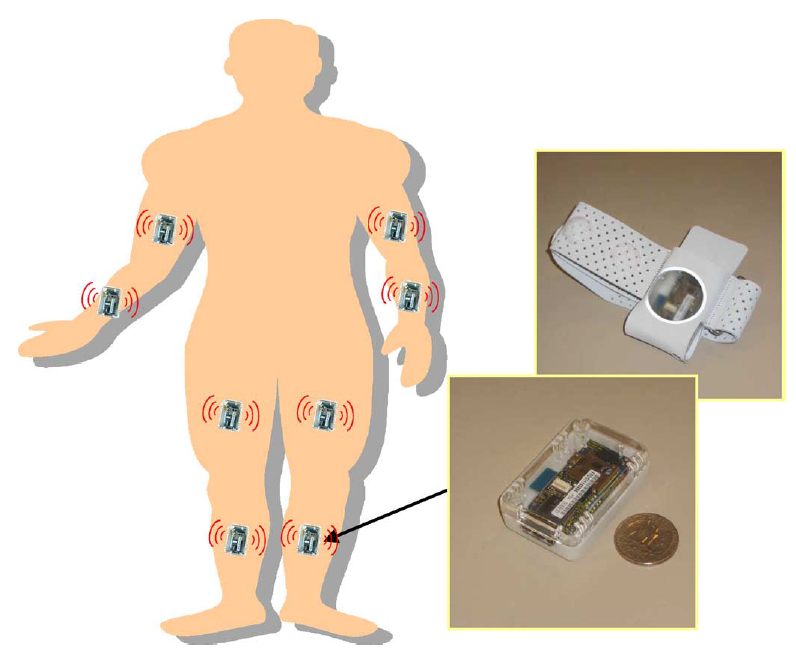
\includegraphics[scale=0.3]{./img/patel-shimmer.png}
 % matrixargseg.png: 296x162 pixel, 100dpi, 7.52x4.11 cm, bb=0 0 213 117
 %\caption{Estágio desenvolvimento de jogos ~\cite{fullerton2008game}}
\caption[Disposição dos Sensores de Movimento (SHIMMER) no corpo no trabalho de Patel]{\textit{Disposição dos Sensores de Movimento (SHIMMER) no corpo no trabalho de Patel ~\cite{patel_monitoring_2009}}}
%  \caption{Estágio desenvolvimento de jogos}
 \label{fig:patel-shimmer}
\end{figure}

\begin{figure}
 \centering
 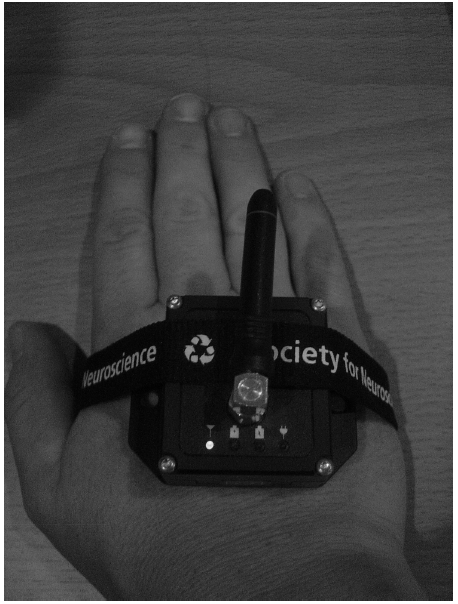
\includegraphics[scale=0.3]{./img/quantif-parkinson.png}
 % matrixargseg.png: 296x162 pixel, 100dpi, 7.52x4.11 cm, bb=0 0 213 117
 %\caption{Estágio desenvolvimento de jogos ~\cite{fullerton2008game}}
\caption[\textit{G-Link Wireless Accelerometer} - Instrumento usado no trabalho de LeMoyne para quantificar o tremor da Doença de Parkinson]{\textit{G-Link Wireless Accelerometer} - Instrumento usado no trabalho de LeMoyne~\cite{LeMoyne2009} para quantificar o tremor da Doença de Parkinson} 
%  \caption{Estágio desenvolvimento de jogos}
 \label{fig:quantif-parkinson}
\end{figure}


Em trabalhos relacionados, LeMoyne~\cite{lemoyne2010} quantificou os sinais de tremores do~\ac{dp} usando um \textit{smartphones}(Figura \ref{fig:iphone-tremor}). LeMoyne~\cite{lemoyne2010} considerou que os \textit{smartphones} estão presentes na rotina dos pacientes e que estes iriam mensurar seus tremores em diferentes momentos do dia. No entanto, o principal problema em mensurar o tremor usando \textit{smartphones} é que o tremor do~\ac{dp} é de repouso~\cite{jankovic2008}. Logo, os pacientes reduzem drasticamente o sinal, o que impacta diretamente na coleta dos dados. Deve-se considerar também que LeMoyne~\cite{lemoyne2010} não realizou avaliações com pacientes ou estudo de caso-controle. 

%TODO: negar mais veementemente
%Em nossos estudos, com o uso dos acelerômetros de celulares junto aos pacientes com~\ac{dp}, identificamos que o tremor foi reduzido drasticamente, porque estes pacientes entravam em modo de ação~\cite{jankovic2008}.

\begin{figure}
 \centering
 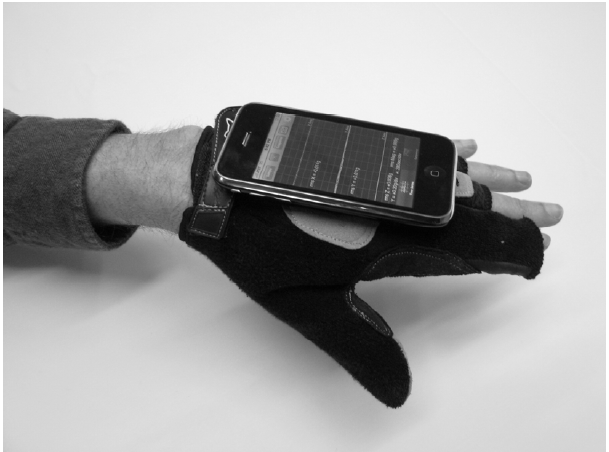
\includegraphics[scale=0.3]{./img/moyne-iphone.png}
 % matrixargseg.png: 296x162 pixel, 100dpi, 7.52x4.11 cm, bb=0 0 213 117
 %\caption{Estágio desenvolvimento de jogos ~\cite{fullerton2008game}}
\caption[Aplicação para \textit{smartphone} com a finalidade de identificar sinais de tremor]{Aplicação para iPhone com a finalidade de identificar sinais de tremor ~\cite{lemoyne2010}}
%  \caption{Estágio desenvolvimento de jogos}
 \label{fig:iphone-tremor}
\end{figure}


\section{Objetivos}
\subsection{Objetivo Principal}
Nesta tese, tem-se como objetivo principal a concepção de uma abordagem computacional não invasiva para o monitoramento de sinais motores. Pretende-se usar jogos eletrônicos como forma de \textbf{motivar} o monitoramento dos sinais motores e abstrair do contexto de \textbf{tratamento da saúde}.

Para atingir esse objetivo, pretende-se desenvolver um~\ac{sms} capaz de: armazenar, processar sinais biomecânicos e identificar a presença do sinal de bradicinesia do~\ac{dp}. 


Para atingir o objetivo principal da pesquisa subdividimos este trabalho em etapas:
	\begin{description}
	\item[ETAPA 1] Quais os benefícios de acompanhar os sinais motores do paciente diariamente, do ponto de vista do profissional da saúde?
	\item[ETAPA 2] Como melhor adquirir e quantificar sinais motores utilizando sensores de movimento para monitorar os sinais do~\ac{dp}?
	\item[ETAPA 3] Avaliar a perspectiva dos usuários quanto à abordagem de quantificar os sinais motores de uma maneira não-invasiva e aplicável à rotina diária.
	\end{description}

\section{Metodologia}
A metodologia de pesquisa deste trabalho possui aspectos qualitativos e quantitativos. Referente ao aspecto qualitativo, buscou-se identificar a importância desta tese junto à comunidade de especialistas da área de saúde. Nos aspectos quantitativos, demonstramos que a abordagem definida consegue diferenciar indivíduos diagnosticados com~\ac{dp} perante indivíduos sem o diagnóstico estabelecido, por meio de dados capturados por sensores de movimento usados em jogos. Ao final do trabalho avaliamos a aceitabilidade da proposta na perspectiva do usuário, utilizando uma análise~\ac{gqm}~\cite{van1999goal}. 

\subsection{Etapas da Pesquisa}
\begin{enumerate}

\item{Realizar revisão bibliográfica e coleta de requisitos junto a profissionais de saúde.}

\item{Definir a abordagem de um~\ac{jogue-me}, baseada em captura de sinais motores através de sensores de movimento, utilizando jogos eletrônicos e processamento dos sinais para transformá-los em informações de saúde.}
%Pode ser também GAME-HMS-E (Game with a Health Monitoring System Embedded)

\item{Analisar a perspectiva dos profissionais de saúde em relação ao acompanhamento dos sinais motores dos pacientes com~\ac{dp} (os profissionais foram indagados sobre a melhora na tomada de decisão quanto ao acompanhamento dos sinais) e verificar se os parâmetros motores, como velocidade angular e amplitude do movimento dos braços, são importantes para realizar o acompanhamento dos sinais do~\ac{dp}. Procurou-se encontrar, junto ao profissional de saúde, a importância do monitoramento dos sinais motores e os benefícios trazidos por este, através de uma abordagem de pesquisa qualitativa. Com esta pesquisa, foi possível validar a \textbf{ETAPA 1}, que consiste em verificar a importância do acompanhamento de sinais motores integrados à rotina diária do paciente.}

\item{Validar o uso de sensores para classificação dos dados através da classificação dos sinais motores adquiridos por sensores de movimento utilizados em jogos eletrônicos. A classificação consistiu em aplicar os sinais numa~\ac{svm} para distinguir indivíduos do grupo controle ante indivíduos diagnosticados com~\ac{dp};
O resultado dessa pesquisa demonstrou a viabilidade da abordagem e, consequentemente, validou a \textbf{ETAPA 2} do trabalho.

\item{Definir a arquitetura de software que viabilizou tecnicamente a abordagem~\ac{jogue-me}. Nesta etapa, definimos um arcabouço de software para encapsular o desenvolvimento de jogos com essa abordagem.}

\item{Validar a solução~\ac{jogue-me} do ponto de vista computacional. A solução foi validada através da implementação da arquitetura e do desenvolvimento de jogos. Com esta etapa, demonstrou-se ser possível realizar monitoramento de dados motores de forma não invasiva, ou seja, sem os jogadores perceberem que estão fornecendo dados de saúde.}

\item{Verificar junto ao público alvo (Pacientes portadores de~\ac{dp}) os requisitos de usabilidade, adequação à rotina diária, segurança física e se a proposta é considerada invasiva na perspectiva do paciente. Com esta avaliação, buscamos validar a \textbf{ETAPA 3} da pesquisa.}

    
%\item{Definir um conjunto de atividades que permitam o desenvolvimento de jogos voltados para o monitoramento de dados de saúde (\ac{jogue-me}). Desta maneira, pretende-se com esse trabalho disseminar o conhecimento adquirido a partir de um conjunto de passos que tornem exequível o desenvolvimento de um \ac{jogue-me}.}

\end{enumerate}

%\subsection{Desenho da Pesquisa} \label{sec:desenho_pesquisa}
%Para uma melhor compreensão da pesquisa temos o Desenho da Pesquisa a ser realizada na Figura \ref{figure:desenho_pesquisa} e a descrição de cada um dos passos.
%
%A Problemática desse trabalho, já foi descrita na Seção \ref{section:problematica}. A revisão da literatura consistiu de uma descrição sobre a doença estudada como estudo de caso (Doença de Parkinson) que está descrito no Capítulo \ref{section:doenca_parkinson}, bem como da possibilidade de integrar o monitoramento da doença de Parkinson por intermédio de jogos eletrônicos.
%
%\begin{figure}[!htp]
    %\centering
    %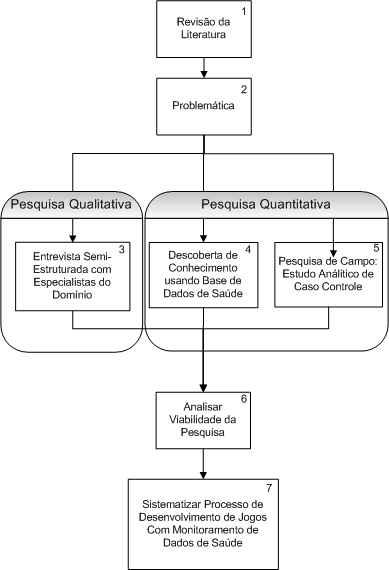
\includegraphics[width=.7\textwidth]{./img/metodologia-pesquisa.png}
    %\caption{Desenho da Pesquisa}
    %\label{figure:desenho_pesquisa}
%\end{figure}

%\subsection{Pesquisa Qualitativa}
%Essa pesquisa tem como objetivo identificar a importância de realizar o monitoramento de dados de saúde por intermédio jogos eletrônicos. Em um primeiro momento, serão verificados junto a comunidade médica a relevância desse trabalho e se este poderia auxiliar no monitoramento dos sinais parkinsonianos.
%
%Os pesquisadores que adotam a abordagem da pesquisa qualitativa a fazem por sua flexibilidade, sem regras rígidas, aplicáveis a uma ampla gama de casos e formalizações pré-definidas, possibilitando a construção de modelos abrangentes \cite{Gom00}.
%Nesse estudo a pesquisa qualitativa está orientada a um estudo de caso, partindo da análise das expressões e comportamento das pessoas. Na busca por entender os fenômenos sociais complexos, o estudo de caso permite uma investigação significativa nas mudanças desses processos\cite{Yin05}.
%
%\subsubsection{Entrevista Semi-Estruturada Com Especialistas do Domínio (3)}\label{section:entrevista_semi-estruturada}
%
%O objetivo deste procedimento foi entender como é feito o acompanhamento dos sinais da doença de parkinson juntamente aos profissionais de saúde (neurologistas que prescrevem a dosagem medicamentosa e fisioterapeutas que fazem o acompanhamento motor do paciente ao longo de seu tratamento). Os mesmos foram indagados se poderia haver melhora na tomada de decisão caso eles pudessem acompanhar o surgimento dos sinais em diferentes momentos do dia por intermédio de um monitoramento frequente dos sinais. Procurou-se encontrar dentro do contexto de estudo, a importância do monitoramento de dados de saúde e os benefícios trazidos por este.
%
%As entrevistas foram realizadas de maneira presencial, onde primeiramente fez-se perguntas não estruturadas e havendo uma maior estruturação no decorrer da entrevista com a preocupação de que seja evitada a referência do entrevistador seja sobre os pontos de vista do entrevistado conforme prega o método científico \cite{FLI04}. Durante a pesquisa foi utilizado recursos de gravação, de modo a facilitar a transcrição dos dados coletados.
%
%\subsection{Descoberta de Conhecimento usando Base de Dados de Saúde}
%Para esse estudo, foram utilizados dados do \textit{PhysioBank} ~\cite{physionet}. O \textit{PhysioBank} armazena sinais fisiológicos e dados relacionados a comunidade de pesquisa biomédica, incluindo sinais vitais, motores de indivíduos saudáveis e de pacientes com uma variedade de sinais como distúrbios neurológicos ou envelhecimento.
%
%A análise dos dados da \textit{Parkinson Disease Database} ~\cite{physionet}, incluiu 50 pacientes de Parkinson e 50 indivíduos que não possuíam desenvolvido a doença (segundo as informações fornecidas pela própria base de dados). Foram calculados, normalizados e escalonados em 80 \textit{frames} um total de 120 ciclos de marcha (Seção \ref{section:analise_marcha}) que foram usados para efetuar a técnica de aplicar a técnica \textit{eigengaits} ~\cite{medeiros2013} que é uma adaptação da Análise dos Componentes Principais que será explicada na Seção \ref{section:analise_marcha_pca}.
%
%\subsection{Estudo Analítico Caso Controle com \textit{Support Vector Machine} (SVM)}
%Esta etapa da pesquisa foi pautada pelo protocolo de pesquisa submetido à avaliação do Comitê de Ética da UFCG, somente após a aprovação deste (\textbf{CAAE: 14408213.9.1001.5182}) é que os dados foram coletados.
%Os resultados que se desejou alcançar com a pesquisa foi o descobrimento de mecanismos para a identificação e classificação de duas classes de indivíduos os  diagnosticados com a doença de parkinson ante indivíduos sem o diagnóstico estabelecido. Durante a pesquisa também analisou-se o sensor de movimento MS-Kinnect ~\cite{kinnect2013} para avaliar a possibilidades de aquisição de dados de saúde baseada na Cinemática Linear do Movimento Humano.
%
%O propósito dessa classificação é explorar a possibilidade de obter dados de saúde de forma contínua e não invasiva a partir de um sensor de captura de movimento usado em jogos eletrônicos (Ms-Kinnect).
%Os dados adquiridos foram processados extraindo características do movimento angular e postos em uma máquina de de Aprendizagem do tipo \textit{Suppport Vector Machine} para realizar a classificação das duas classes de dados.

\section{Trabalhos Relacionados}\label{section:jogos_saude}

Devido ao estilo de vida mais sedentário e ao aumento da população obesa, as pesquisas para a promoção da atividade física têm se tornado tópico de interesse para a comunidade científica~\cite{maitland2009,bartolome11,Mandryk2014}. Estudos demostram que uma atividade física regular traz benefícios físicos, cognitivos e emocionais~\cite{Mandryk2014}. Com o surgimento dos jogos comerciais, como o \textit{Wii Sports} da Nintendo~\footnote{http://www.nintendo.com}, em 2006, que aumentou a prática de atividade física de jogadores considerados sedentários~\cite{wiigraves2008}, é que pesquisadores da área de jogos para saúde buscaram apoiar essa prática com desenvolvimento de aplicações que motivassem a prática de atividade física~\cite{stacey2011}. Atualmente, os dispositivos de sensores de movimento permitem desenvolver jogos que promovem a saúde e o bem estar de forma promissora. Por esse motivo, houve um aumento significativo de jogos comerciais com o propósito de promover a saúde e o bem-estar da população~\cite{Papastergiou:2009:EPC:1570538.1570707}.


Os jogos pervasivos móveis motivam a atividade física de forma mais direta, tais como: \textit{Transe}, \textit{Feeding Yoshi} e  \textit{Nokia Wellness Diary and Sports Tracker} promovem a saúde com a prática de atividade física~\cite{Suhonen:2008:SFE:1457199.1457204} e melhoram as condições de saúde por serem divertidos, imersivos e engajados. Para o público idoso, foram desenvolvidos diferentes jogos para a melhora da saúde, como: sistemas para reabilitação motora dos idosos~\cite{brox11} e também para pacientes com~\ac{dp}~\cite{atkinson2010,synnott_wiipd_2012,sacbespoke2014}. 

Atkinson e Narasimhan~\cite{atkinson2010} desenvolveram um jogo que utiliza um sensor de toque para quantificar a habilidade motora do paciente com~\ac{dp}. Teoricamente, esta abordagem auxilia no diagnóstico do~\ac{dp}. No entanto, não foi realizado nenhum estudo com os pacientes para avaliar sua eficácia. Synnott \textit{et al.}~\cite{synnott_wiipd_2012} desenvolveu um sistema de gerenciamento medicamentoso e um jogo, utilizando um sensor de captura de movimentos, para identificar o sinal de tremor do~\ac{dp}. No entanto, o tremor do~\ac{dp} é de repouso~\cite{national2006parkinson}. Logo, quando o usuário está concentrado, entra no estado de ação e reduz drasticamente o tremor.

Papastergiou \textit{et al.}~\cite{Papastergiou:2009:EPC:1570538.1570707} identificou efeitos positivos para a reabilitação através do uso do jogo \textit{Wii Sports} e um potencial mecanismo de prevenção e reeducação motora com o uso do \textit{Wii Fit}. Porém, esses jogos possuem suas limitações e não são substitutos dos esportes reais. Ainda assim, o autor salienta que um ambiente mais controlado, que permite a execução de atividades físicas, inibe a ocorrência de situações de risco como um movimento brusco e que venha causar um dano físico maior. Baseado nessas observações, esse trabalho primou por demonstrar as dificuldades e os efeitos positivos em combinar os jogos sérios de esportes e saúde com as tecnologias de sensores, para a personalização e adaptação dos jogos. Paraskevopoulos \textit{et al.}~\cite{sacbespoke2014} propõe um conjunto de diretrizes para o desenvolvimento de jogos com o objetivo de acompanhar o tratamento fisioterápico dos pacientes com~\ac{dp} e dar suporte à reabilitação destes.

Sinclair \textit{et al.}~\cite{Sinclair:2009:UVB:1515604.1515617} considera que os jogos comerciais para prática de exercício físico (\textit{exergames}) não devem ser usados apenas como um motivador para a prática, mas também podem ser usados para monitorar sinais vitais como batimento cardíaco e reconhecer atividades via acelerômetros. Arntzen~\cite{arntzen2011} se preocupou com os aspectos cognitivos e físicos da aprendizagem baseada em jogos para idosos~\cite{arntzen2011}, defendendo que é necessário identificar quais habilidades cognitivas e físicas precisam ser desenvolvidas, além de considerar a limitação do idoso em relação aos movimentos bruscos no intuito de evitar lesões.

Nesta tese, propomos monitorar os pacientes de~\ac{dp} de uma forma não invasiva, por intermédio de sensores de movimento, usando jogos eletrônicos para motivar a aquisição dos sinais e fazendo com que os usuários se abstraiam do tratamento, de forma a não perceber que estão em tratamento. Logo, nosso principal objetivo foi prover um mecanismo de monitoramento dos sinais motores, em um ambiente lúdico e descontraído como um jogo eletrônico.


\section{Contribuições}
Atualmente, os jogos são aplicados para melhora da saúde em diferentes contextos. No entanto, nenhum dos trabalhos relacionados pretendem identificar sinais para monitorar o estado de saúde. Logo, este trabalho visa desenvolver um ambiente de jogo que motive a execução de movimentos específicos, com o propósito de quantificar os sinais motores dos usuários.

No entanto, alinhar a jogabilidade e a capacidade de monitoramento dos sinais de saúde não é trivial, pois deve ser levado em consideração o uso dos sensores e deve-se definir quais movimentos ou ações permitem a identificação dos sinais motores. Por este motivo, a proposta de um~\ac{sms} dos sinais motores usando jogos necessita de um acompanhamento de um profissional de saúde para supervisionar e auxiliar nas definições dos movimentos e ações dos usuários. 

%Posteriormente, na posse dessas ações, deverá ser testada a execução dessas atividades e sua aquisição para uma possível classificação dos dados conforme proposto nesta tese.
%os trabalhos já existentes~\cite{Ballegaard:2008:HEL:1357054.1357336,patel_monitoring_2009,visionbased2009,bachlin_parkinsons_2009,albanese2012}.
%De posse dos movimentos e da captura dos dados será feito um levantamento de um \textit{game design} que permita executar os movimentos em  um ambiente lúdico e divertido como um jogo para entretenimento ~\cite{sweetser2005-gameflow}.

Como possível cenário de uso para a pesquisa, supondo que um paciente de uma doença crônica como o~\ac{dp} faz uso de medicamento antiparkinsoniano e possui um jogo de monitoramento de sinais do~\ac{dp} em sua residência, caso ele utilize o jogo em diferentes momentos do dia, os sinais podem ser quantificados sem a presença de um profissional de saúde, que poderia visualizar a melhora ou piora do estado de saúde do seu paciente ao longo dos dias. A partir da presente abordagem, o médico, ao possuir a informação, poderia gerenciar melhor a dosagem medicamentosa e, consequentemente, prolongar a qualidade de vida do paciente~\cite{rodrigues2006}.

\section{Organização do Documento}
O restante deste documento está organizado da seguinte forma:
\begin{itemize}
	\item No Capítulo~\ref{chapter:fundamentacao} está descrita a fundamentação teórica relacionada ao trabalho.
	\item No Capítulo~\ref{chapter:abordagem_gahme} está definida a abordagem \ac{jogue-me} de monitoramento de sinais motores não invasivo usando jogos eletrônicos.
	\item No Capítulo~\ref{chapter:arquitetura_captura} é demonstrada uma implementação da abordagem.
	\item No Capítulo~\ref{chap:avaliacao} são apresentados os experimentos realizados para validar a tese.
	\item No Capítulo~\ref{chapter:conclusoes_futuros} são apresentadas as conclusões do trabalho e propostos trabalhos futuros.
\end{itemize}
